% 两点距离公式推导：A(x1,y1), B(x2,y2), C(x2,y1) 构成直角三角形
\documentclass[tikz,border=4pt]{standalone}
\usepackage{ctex}
\usepackage{amsmath}
\usetikzlibrary{calc}
\begin{document}
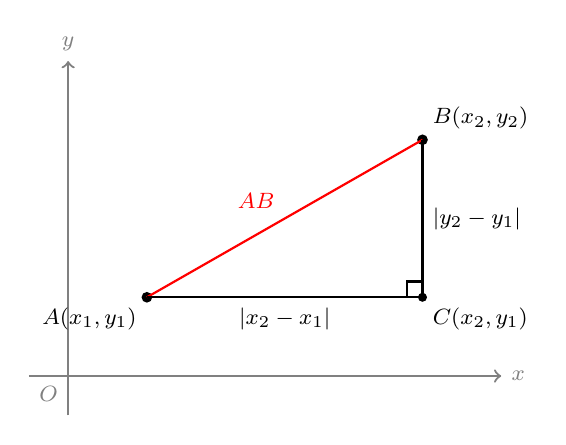
\begin{tikzpicture}[thick, scale=1.0]
  \draw[->, gray] (-0.5,0) -- (5.5,0) node[right, font=\footnotesize] {$x$};
  \draw[->, gray] (0,-0.5) -- (0,4) node[above, font=\footnotesize] {$y$};
  \node[font=\footnotesize, below left, gray] at (0,0) {$O$};
  % A 在 (1,1), B 在 (4.5,3)
  \coordinate (A) at (1,1);
  \coordinate (B) at (4.5,3);
  \coordinate (C) at (4.5,1);
  \filldraw (A) circle (1.5pt) node[below left, font=\footnotesize] {$A(x_1,y_1)$};
  \filldraw (B) circle (1.5pt) node[above right, font=\footnotesize] {$B(x_2,y_2)$};
  \filldraw (C) circle (1.2pt) node[below right, font=\footnotesize] {$C(x_2,y_1)$};
  \draw[red, thick] (A) -- (B);
  \draw[thick] (A) -- (C);
  \draw[thick] (C) -- (B);
  % 直角标记
  \draw (4.3,1) -- (4.3,1.2) -- (4.5,1.2);
  \node[font=\footnotesize, below] at ($(A)!0.5!(C)$) {$|x_2-x_1|$};
  \node[font=\footnotesize, right] at ($(C)!0.5!(B)$) {$|y_2-y_1|$};
  \node[font=\footnotesize, above left, red] at ($(A)!0.5!(B)$) {$AB$};
\end{tikzpicture}
\end{document}
